\newpage
\section{Abstract syntax and static semantics}
\genHeader
\label{sec: staticSemantics}

The first step in creating any metamodel is defining the abstract syntax, also known as the type graph. This involves defining each class, its attributes,
references, and method signatures.

If you completed the demo in Part I, your Eclipse workspace will look slightly different than ours depicted in the screenshots. In an effort to keep things as
clear as possible, we have removed those files from our package explorer, but still recommend keeping them for future reference. 

Additionally, if you're continuing from the visual demo, you can begin modeling this project in two different ways. You can either develop your metamodel in
the same workspace as the demo, or create a new one. Either way, please note that the steps are exactly the same, but our project browsers in
EA may not exactly match. This handbook has assumed you prefer the latter.

\jumpDual{static:starting vis}{static:starting tex}

\newpage
\subsection{Getting started in EA}
\visHeader
\hypertarget{static:starting vis}{}
  
{\bf Note:} To continue with Part I's Demo files, open the \texttt{demo.eap} file in EA, initialise a new diagram, then work within that EA project. You can
ignore the first instruction below. (test this!)

\begin{itemize}

\item[$\blacktriangleright$]  To begin, navigate to ``New Metamodel Project,'' and start a new visual project (this time without the demo specifications)
named \texttt{Leit\-ners\-Learn\-ing\-Box} (Fig.~\ref{fig:new_visModel}). Open the empty \texttt{.eap} file in EA.

\vspace{0.5cm}

\begin{figure}[htbp]
	\centering
  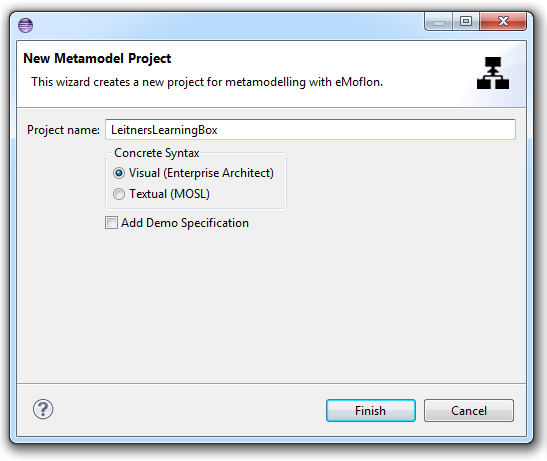
\includegraphics[width=0.8\textwidth]{eclipse_visNewMetamodelPlain}
	\caption{Starting a new visual project}
	\label{fig:new_visModel}
\end{figure}

\vspace{0.5cm}

\item[$\blacktriangleright$] In EA, select your working set and press the ``Add a Package'' button (Fig.~\ref{fig:new_package}). (test: make sure
\texttt{eMoflonLanguages} is included in BOTH new file and Demo specs. (gotta look the same!) )

\begin{figure}[htbp]
	\centering
  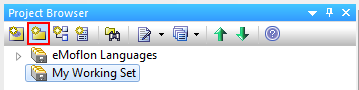
\includegraphics[width=0.5\textwidth]{ea_addPackage}
	\caption{Add a new package to \texttt{MyWorkingSet}}
	\label{fig:new_package}
	\vspace{0.5cm}
\end{figure}

\clearpage

\item[$\blacktriangleright$] In the dialogue that pops up (Fig.~\ref{fig:new_package_name}), enter \texttt{LearningBoxLanguage} as the name of the new
package. Make sure \texttt{Class View} is selected, and click \texttt{OK}.

\vspace{0.5cm}

\begin{figure}[htbp]
	\centering
    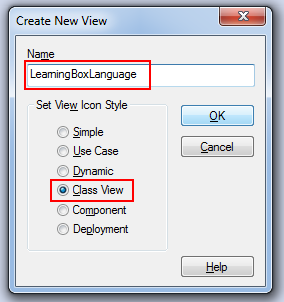
\includegraphics[width=0.33\textwidth]{ea_nameEPackage.png}
	\caption{Enter the name of the new package}
	\label{fig:new_package_name}
\end{figure}
\FloatBarrier

\vspace{0.5cm}

\item[$\blacktriangleright$] Your \texttt{Project Browser} should now resemble Fig.~\ref{fig:new_package_completed}.

\vspace{0.5cm}

\begin{figure}[htbp]
	\centering
  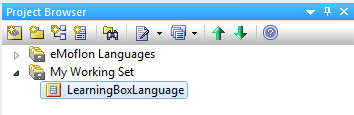
\includegraphics[width=0.5\textwidth]{ea_newPackage}
	\caption{State after creating the new package.}
	\label{fig:new_package_completed}
\end{figure}
\FloatBarrier


\vspace{0.5cm}

\item[$\blacktriangleright$] Now select your package and create a ``New Diagram'' (Fig.~\ref{fig:diagram}).

\vspace{0.5cm}

\begin{figure}[htbp]
	\centering
  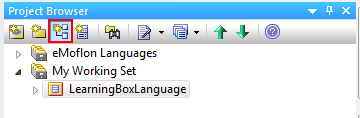
\includegraphics[width=0.5\textwidth]{ea_addDiagram}
	\caption{Add a diagram.}
	\label{fig:diagram}
\end{figure}
\FloatBarrier

\clearpage

\item[$\blacktriangleright$] In the dialogue that appears (Fig.~\ref{fig:diagram_type}), choose \texttt{eMoflon Ecore Diagrams} and press \texttt{OK}. 

\begin{figure}[htbp]
	\centering
  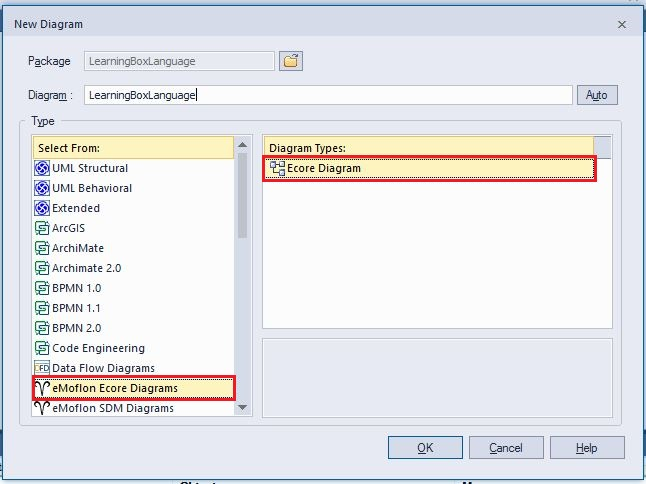
\includegraphics[width=0.8\textwidth]{ea_chooseDiagramType}
	\caption{Select the ecore diagram type}
	\label{fig:diagram_type}
\end{figure}
\FloatBarrier

 
\item[$\blacktriangleright$] After creating the new diagram, your  \texttt{Project Browser} should now resemble Fig.~\ref{fig:diagram_completed}. You'll notice
that your \texttt{LearningBoxLanguage} package has been transformed into an EPackage.

\begin{figure}[htbp]
	\centering
  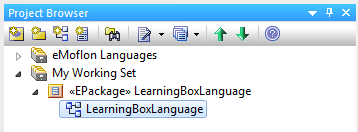
\includegraphics[width=0.5\textwidth]{ea_afterDiagramState}
	\caption{State after creating diagram}
	\label{fig:diagram_completed}
\end{figure}
\FloatBarrier

\item[$\blacktriangleright$] You can now already export your project to Eclipse,\footnote{If unsure how to perform this step, please
refer to Part I, section 2.1} then refresh your \texttt{Package Explorer}. A new node, \texttt{My Working Set}\footnote{If you do not have the two
distinct nodes, make sure your ``Top Level Elements'' are set to \texttt{Working Sets}} should have appeared containing your \texttt{Epackage}
(Fig.~\ref{fig:init_export}). You can see that a \texttt{LearningBoxLanguage.ecore} file has been generated, and placed in ``model.'' This is your metamodel
that will contain all future types you create in your diagrams.

\clearpage

\vspace*{2cm}

\begin{figure}[htbp]
	\centering
  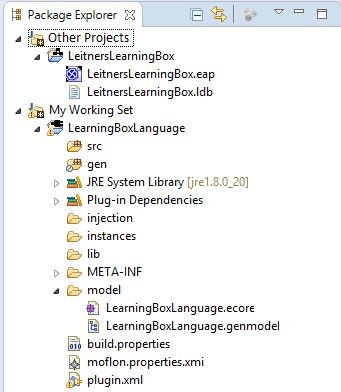
\includegraphics[width=0.55\textwidth]{eclipse_visInitExport}
	\caption{Inital export to Eclipse}
	\label{fig:init_export}
\end{figure}

\vspace{1cm}

\item[$\blacktriangleright$] If you're interested in reviewing the overall project structure, the purposes of certain files and folders, read section 4.1 from
Part~I\footnote{Download link: \dlPartOne} of this handbook. Otherwise, continue to the next to section learn how to declare classes and attributes.

\fancyfoot[R]{$\triangleright$ \hyperlink{static:classes vis}{Next}}
\end{itemize}

\clearpage
\subsection{Getting started with MOSL}
\texHeader
\hypertarget{static:starting tex}{} 

\begin{itemize}

\item[$\blacktriangleright$] Create a new metamodel project in Eclipse by navigating to the \texttt{New Metamodel} button in the toolbar. In the dialogue that
appears, enter \texttt{LeitnersLearningBox} as the project name, and select \texttt{Textual (MOSL)}  (Fig.~\ref{eclipse:newProject}).

\vspace{1cm}

\begin{figure}[htbp]
	\centering
  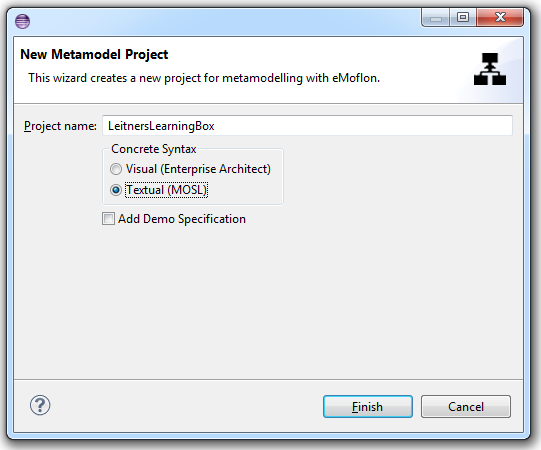
\includegraphics[width=0.8\textwidth]{eclipse_texNewMetamodelPlain}
	\caption{Creating a new metamodel project}
	\label{eclipse:newProject}
\end{figure}

\vspace{1cm}

\item[$\blacktriangleright$] You'll see your new project appear under the ``Specifications" node.\footnote{If no nodes appear in your package explorer,
ensure your ``Top Level Elements'' are set to ``WorkingSets''} If you're interested in the details of eMoflon's project structure, review Section
4.2 from Part I. Otherwise, expand the project as deep as it goes (Fig.~\ref{eclipse:expandedFolders}).

\clearpage

\begin{figure}[htbp]
	\centering
  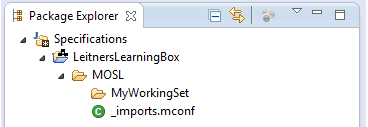
\includegraphics[width=0.6\textwidth]{eclipse_texFoldersExpanded}
	\caption{Expanded project files}
	\label{eclipse:expandedFolders}
\end{figure} 

\vspace{0.5cm}

\item[$\blacktriangleright$] We're most interested in \texttt{MOSL/MyWorkingSet}, which represents the project scope. Right click this folder, and create a new
\texttt{EPackage} (Fig.~\ref{eclipse:newEPackage}), naming it \texttt{LearningBoxLanguage}. Using this wizard to generate your EPackage will automatically
create the necessary \texttt{\_patterns} folder and \texttt{\_constraints} file.

\vspace{0.5cm}

\begin{figure}[htbp]
	\centering
  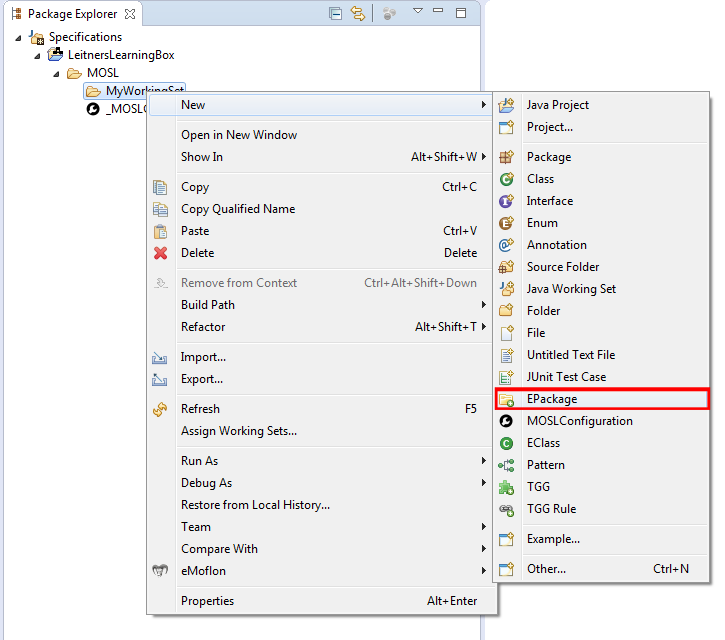
\includegraphics[width=0.8\textwidth]{eclipse_newEPackage}
	\caption{Create an EPackage in your working set}
	\label{eclipse:newEPackage}
\end{figure} 

\clearpage

\item[$\blacktriangleright$] Your package explorer should now resemble Fig.~\ref{eclipse:preBuild}.

\item[$\blacktriangleright$] To finish initalising your metamodel, navigate to ``Build (Without cleaning),'' found beside ``New Metamodel'' in the
toolbar (Fig.~\ref{eclipse:preBuild}).

\begin{figure}[htbp]
	\centering
  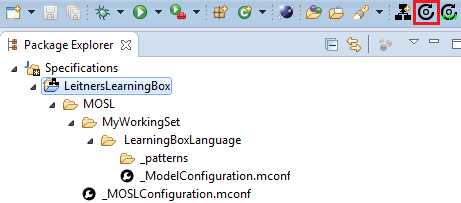
\includegraphics[width=0.6\textwidth]{eclipse_texBuildButton}
	\caption{Inital structure of Leitner's Learning Box}
	\label{eclipse:preBuild}
\end{figure} 

\vspace{0.5cm}

\item[$\blacktriangleright$] A new, ``MyWorkingSet'' node, named after your project container, should have been created (Fig.~\ref{eclipse:finalFiles}). The
folder ``gen'' is where all Java files generated from your metamodel will be placed.

\vspace{0.5cm}

% Forced position at the bottom of the page
\begin{figure}[h!]
	\centering
  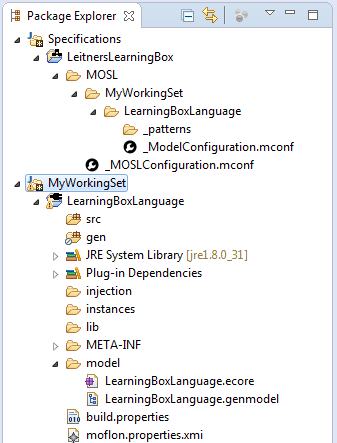
\includegraphics[width=0.5\textwidth]{eclipse_texFinalExpansion}
	\caption{The project fully initialised}
	\label{eclipse:finalFiles}
\end{figure} 

\vspace{0.5cm}

\item[$\blacktriangleright$] Navigate to ``LearningBoxLanguage/model.'' This folder contains \\ \texttt{LearningBoxLanguage.ecore}, your metamodel. This will
contain all types you define in ``LeitnersLearningBox/MOSL/MyWorkingSet/LearningBoxLanguage.''

\item[$\blacktriangleright$] Your project structure is now complete! In the next section, we'll start creating classes and attributes.

\jumpSingle{static:classes tex}

\end{itemize}


\newpage
\subsection{Declaring classes and attributes}
\genHeader
\hypertarget{static:classes vis}{}

\begin{stepbystep}

\item Return to EA, and double-click your \texttt{LearningBoxLanguage} diagram to ensure it's open.

\vspace{0.5cm}

\item There are two ways for you to create your first \texttt{EClass}. First, to the left of the workbench, a \emph{Toolbox} containing
the Ecore types available for metamodelling should have appeared (\Cref{ea:eclass}).\footnote{If not, choose ``Diagram/Diagram Toolbox'' to show the
current toolbox (Alt+ 5)} Click on the \texttt{EClass} icon then somewhere in the diagram to create a new object. Alternatively, you can click in the diagram and press
\texttt{space} to invoke the toolbox context menu, then select \texttt{EClass}.

\vspace{0.5cm}

\begin{figure}[htbp]
	\centering
  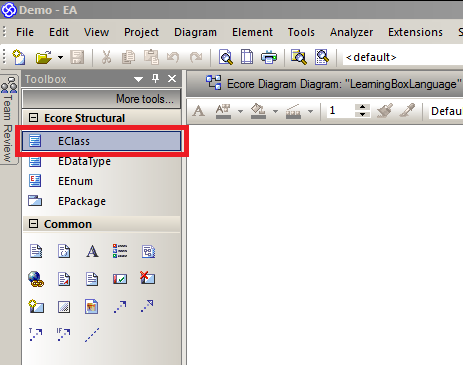
\includegraphics[width=0.7\textwidth]{ea_createEClass}
	\caption{Create an EClass}
	\label{ea:eclass}
\end{figure}

\vspace{0.5cm}

\item In the dialogue that pops-up, set \texttt{Box} as the name and click \texttt{OK} (\Cref{ea:eclass_properties}).
This dialogue can always be invoked again by double-clicking the EClass, or by pressing \texttt{Alt} and single-clicking. It contains many other properties that we'll investigate later in the handbook. In general, a similar properties dialogue can be opened in the same fashion for almost every element in EA.

\clearpage

\begin{figure}[ht]
	\centering
  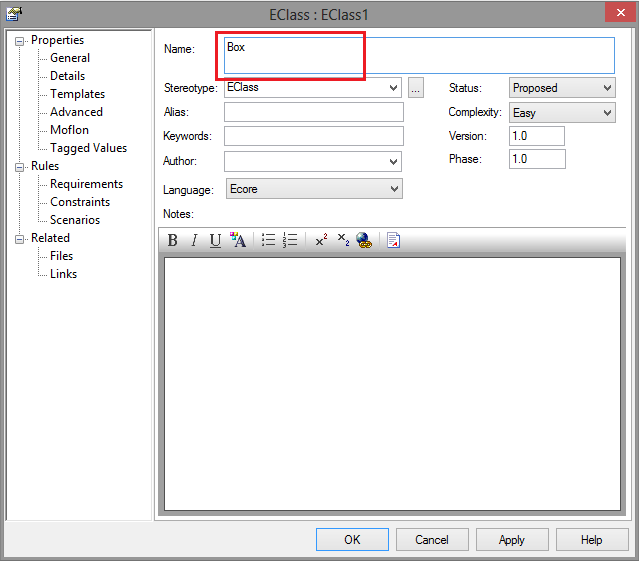
\includegraphics[width=0.9\textwidth]{ea_propertiesEClass}
	\caption{Edit the properties of an EClass}
	\label{ea:eclass_properties}
\end{figure}

\item After creating \texttt{Box}, your EA workspace should resemble \Cref{ea:eclass_completed}.

\vspace{0.5cm}

\begin{figure}[htbp]
	\centering
  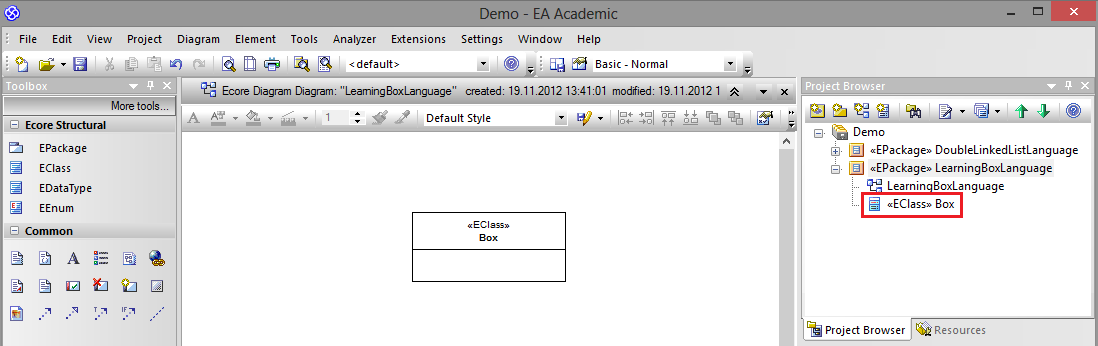
\includegraphics[width=1\textwidth]{ea_afterBoxCreation}
	\caption{State after creating \texttt{Box}}
	\label{ea:eclass_completed}
\end{figure}

\item Now create the \texttt{Partition} and \texttt{Card} EClasses the same way, until your workspace resembles
\Cref{ea:all_eclasses}. These are the main classes of your learning box metamodel.

\vspace{0.5cm}

\item Lets add some attributes! Either right-click on \texttt{Box} to activate the context menu and choose ``Features \&
Properties/Attributes..'' (\Cref{ea:attribute}), or press \texttt{F9} to open the editing dialogue.

\begin{figure}[htbp]
	\centering
  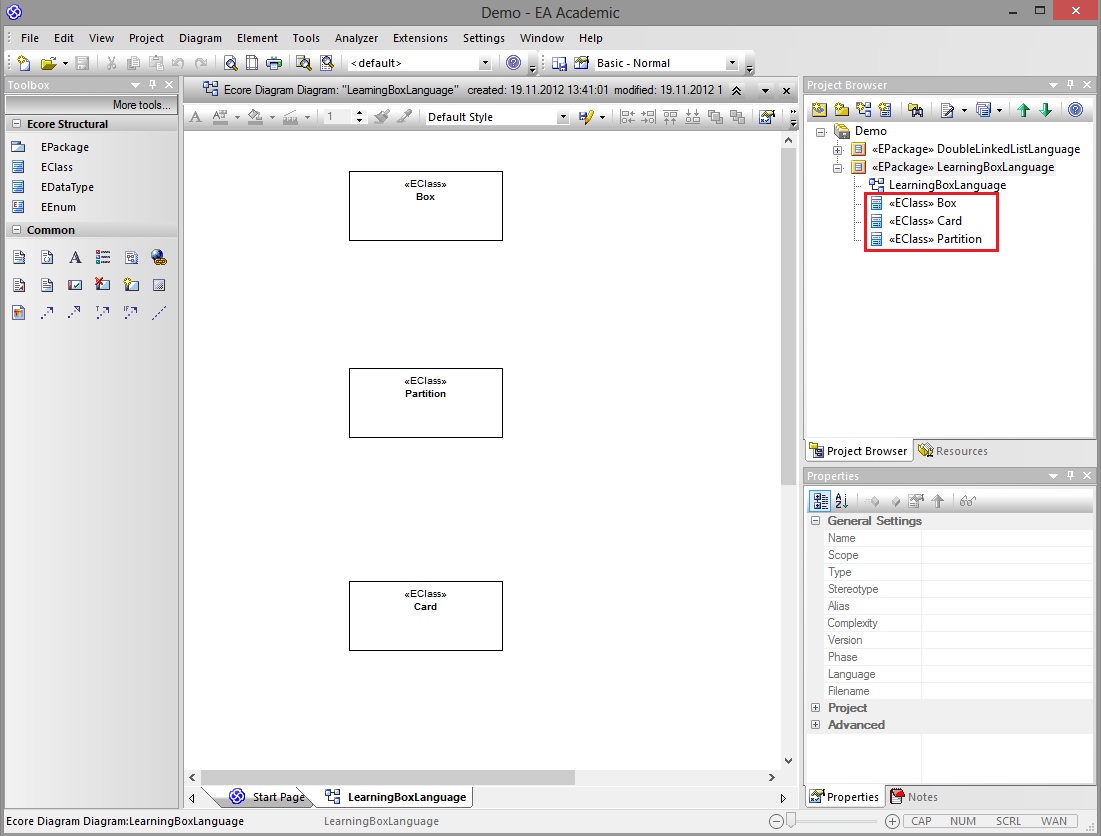
\includegraphics[width=\textwidth]{ea_createPartitionCard}
	\caption{All EClasses for the metamodel}
	\label{ea:all_eclasses}
\end{figure}

\begin{figure}[htbp]
	\centering
  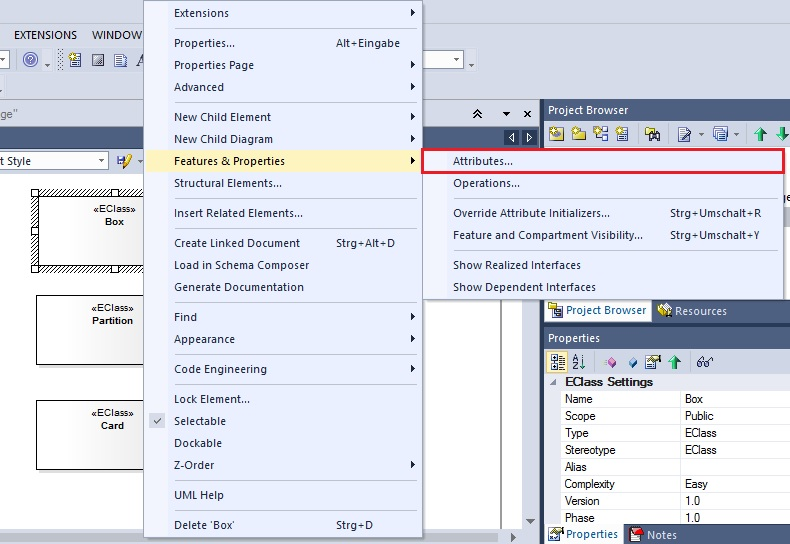
\includegraphics[width=\textwidth]{ea_contextAddAttribute}
	\caption{Context menu for an EClass}
	\label{ea:attribute}
\end{figure}
\FloatBarrier

\item Enter \texttt{name} as the name of the attribute, select \texttt{EString} as its type from the drop-down menu, and press
\texttt{Close} (\Cref{ea:attribute_properties}). New attributes for the same EClass can be added by clicking on \texttt{New Attribute}...\,.

\vspace{1.0cm}

\begin{figure}[htbp]
	\centering
  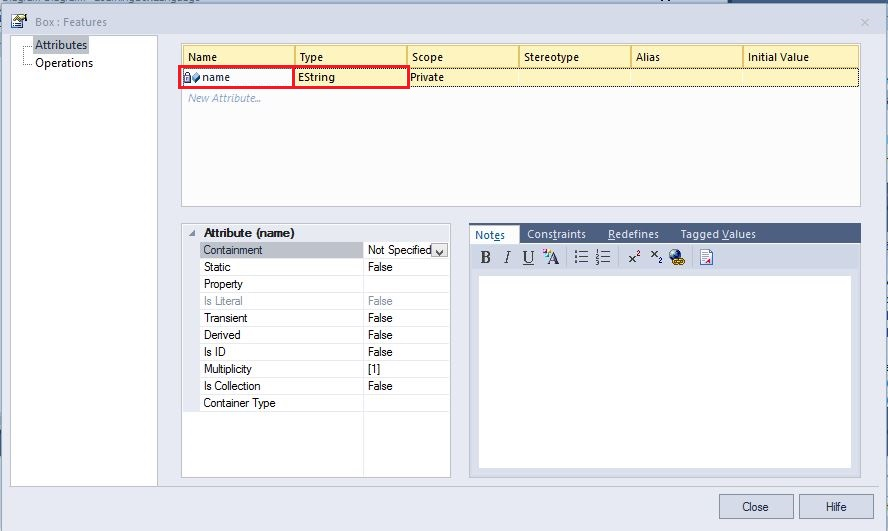
\includegraphics[width=0.9\textwidth]{ea_addAttributesDialogue}
	\caption{Adding attributes to an EClass}
	\label{ea:attribute_properties}
\end{figure}

\vspace{0.5cm}

\item Add the remaining attributes analogously to each EClass until your workspace resembles \Cref{ea:attribute_completed}.

\vspace{0.5cm}

\item Save and export to Eclipse. After refreshing your workspace, your \texttt{.ecore} model can now be expanded as it includes
every class and attribute from your metamodel. So far, so good!

\newpage

\vspace*{3cm}

\begin{figure}[htbp]
	\centering
  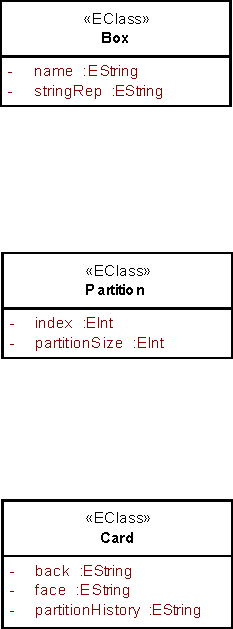
\includegraphics[width=0.40\textwidth]{ea_allAttributes}
	\caption{Main EClasses declared with their attributes}
	\label{ea:attribute_completed}
\end{figure}
\FloatBarrier

\end{stepbystep}

\newpage
\hypertarget{static:classes tex}{}
\subsection{Declaring classes and attributes}
\texHeader

\begin{itemize}

\item[$\blacktriangleright$] Right click your \texttt{LearningBoxLanguage} model and create your first EClass by navigating to ``New/EClass.'' Name it
\texttt{Box}.

\vspace{0.5cm}

\item[$\blacktriangleright$] The class editor should automatically open. Let's add the first two EAttributes of our \texttt{Box}, \texttt{name} and
\texttt{stringRep}. eMoflon offers auto-completion templates to help you with
this task. Go to an empty line and press \texttt{Ctrl + Space}. You'll be
provided with a short list of suggestions (Fig.~\ref{eclipse:typeCompTempl}).
The first four items are related to method control flow, so select \texttt{attribute} near
the bottom to create \texttt{name} of type \texttt{EString}.

\vspace{0.5cm}

\begin{figure}[htbp]
	\centering
  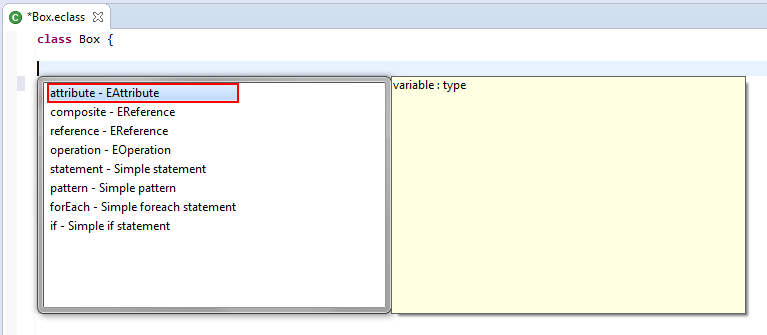
\includegraphics[width=0.6\textwidth]{eclipse_typeCompletionTemplates}
	\caption{eMoflon's auto-completion}
	\label{eclipse:typeCompTempl}
\end{figure} 

\vspace{0.5cm}

\item[$\blacktriangleright$] Auto-completion also supports you by suggesting a list of types. Start to create a second attribute, \texttt{stringRep}, but
stop after typing the \texttt{`:'} operator and press the hotkeys. The pop-up list provides a list of all types currently available
(Fig.~\ref{eclipse:typeCompTypes}) in both your metamodel, and eMoflon's standard metamodels that are included in every new project.

\vspace{0.5cm}

\item[$\blacktriangleright$] Your workspace should now resemble (Fig.~\ref{eclipse:boxDeclaration}).

\newpage

\begin{figure}[htbp]
	\centering
  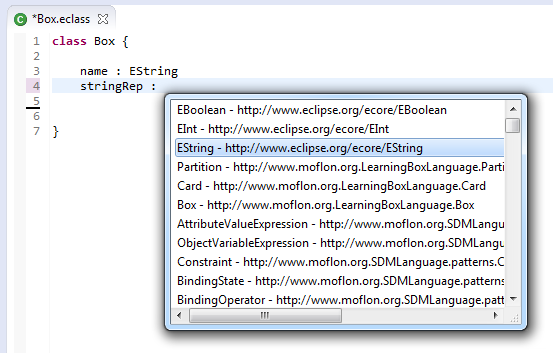
\includegraphics[width=0.6\textwidth]{eclipse_typeCompletionTypes}
	\caption{Type suggestions for \texttt{stringRep}}
	\label{eclipse:typeCompTypes}
\end{figure} 

\vspace{0.5cm}

\begin{figure}[htbp]
	\centering
  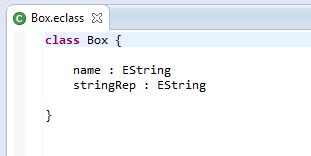
\includegraphics[width=0.5\textwidth]{eclipse_classBoxDeclaration}
	\caption{Newly created \texttt{Box} EClass}
	\label{eclipse:boxDeclaration}
\end{figure} 
\FloatBarrier

\vspace{0.5cm}

\item[$\blacktriangleright$] Now create two empty EClasses in your model, \texttt{Partition} and \texttt{Card}.

\vspace{0.5cm}

\item[$\blacktriangleright$] In \texttt{Partition}, add two \texttt{EInt} attributes, \texttt{index} and \texttt{partitionSize}.

\vspace{0.5cm}

\item[$\blacktriangleright$] In \texttt{Card}, create three \texttt{EString} attributes, \texttt{back}, \texttt{face} , and \texttt{part\-it\-ion\-His\-tory}.

\item[$\blacktriangleright$] If you've done everything correctly, your workspace should now resemble Fig.~\ref{eclipse:workspaceClassAttributes}.

\begin{figure}[htbp]
	\centering
  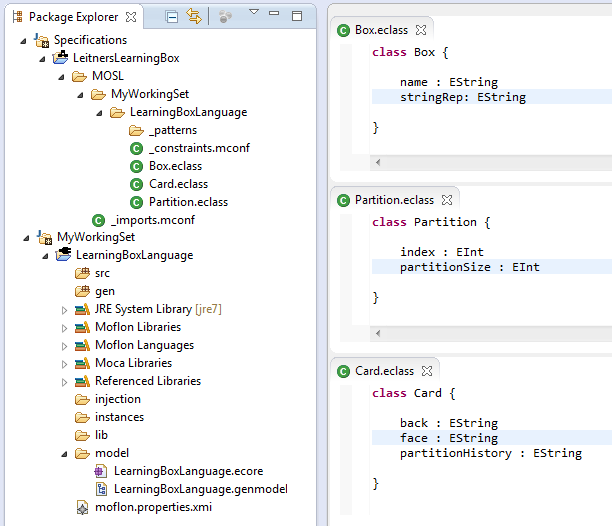
\includegraphics[width=1.0\textwidth]{eclipse_workspaceTexClassAttributes}
	\caption{Declaration of all EClasses and attributes}
	\label{eclipse:workspaceClassAttributes}
\end{figure} 

\vspace{0.5cm}

\item[$\blacktriangleright$] That's it for declaring class attributes! Feel free to build your project again and view the changes in the \texttt{.ecore}
mode, and the generated files in ``gen" and ``src." On a final note, while some languages (such as Java) allow the declaration of several small classes (such as
these three) in the same file, when tooling with eMoflon, we keep them separated. Don't worry -- we'll explain this later in the handbook. As for now, continue
to the next section to start creating references between these EClasses.

\end{itemize}


\newpage
\subsection{Connecting your classes}
\genHeader
\hypertarget{static:references splash}{}

\texttt{}
\emph{}

At this point, you've declared your types and attributes, but what good are those if nothing can communicate with something else? We need to create some
\emph{EReferences}!

There are 3 properties that must be set in order to create an EReference: \emph{Navigation}, \emph{Aggregation}, and
\emph{Multiplicity}. As you can probably guess, they're declared differently in each syntax, but let's review the concepts since they're the same.

Firstly, \texttt{Navigable} ends are mapped to class attributes with getters and setters in Java, and therefore \emph{must} have a specified name and
multiplicity for successful code generation. Corresponding values for \texttt{Non-Navigable} ends can  be regarded as additional documentation, and do not have
to be specified.

Second, the \texttt{Multiplicity} refers to that of a reference\footnote{Don't get multiplicity of a reference confused with the multiplicity of an element!
Multiplicity of an element defines the permitted range of individual instances, rather than classes.}. It controls if the relation is mapped to a
Java Collection (\texttt{*},~\texttt{1..*},~\texttt{0..*}), or to a single valued class attribute (\texttt{1}, \texttt{0..1}). We'll explain this setting in
detail when you encounter them in your syntax instructions.

Lastly, in Ecore, the \texttt{Aggregration} values of a reference can be \texttt{none}, \texttt{shared}, or \texttt{com\-po\-site}. Composite means that the
current role is that of a \emph{container} for the opposite role. You'll see in our example that \texttt{Box} is a container for several \texttt{Partition}s.
This has a series of consequences: (1) every element must have a container, (2) an element cannot be in more than one container at the same time, and (3) a
container's contents are deleted together with the container. Conversely, non-composite (\texttt{none}) means that the current role is not that of a container,
and the rules for containment do not hold (in other words, the reference is set a simple `pointer'). The \texttt{shared} setting is beyond the scope of this
handbook.


\fancyfoot[RO]{ $\triangleright$ \hyperlink{static:references vis}{Next [visual]\hspace{0.2cm}} \\ $\triangleright$ \hyperlink{static:references tex}{Next
[textual]}}

\newpage
\subsubsection{Creating EReferences in EA}
\visHeader
\hypertarget{static:references vis}{}

\begin{itemize}

\item[$\blacktriangleright$] A fundamental gesture in EA is \emph{Quick Link}. Quick Link is used to create EReferences between elements in a context-sensitive
manner. To use quick link, choose an element and note the little black arrow in its top-right corner (Fig.~\ref{fig:quicklink}).

\begin{figure}[htbp]
	\centering
  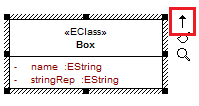
\includegraphics[width=0.4\textwidth]{ea_quickLink}
	\caption{Quick Link is a central gesture in EA}
	\label{fig:quicklink}
\end{figure}
\FloatBarrier

\item[$\blacktriangleright$] Click this black arrow and `pull' to the element you wish to link to. To start, quick-link from \texttt{Box} to \texttt{Partition}.
In the context menu that appears, select ``Create Bidirectional EReference'' (Fig.~\ref{fig:ereference}).

\begin{figure}[htbp]
	\centering
  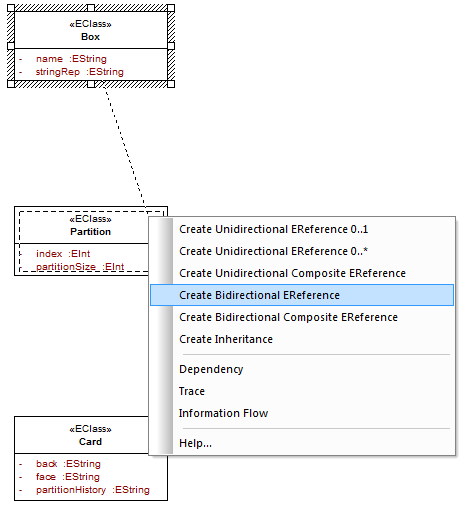
\includegraphics[width=0.6\textwidth]{ea_eReferenceBidirectional}
	\caption{Create an EReference via Quick Link}
	\label{fig:ereference}
\end{figure}
\FloatBarrier

\item[$\blacktriangleright$] Double click the EReference to invoke a dialogue. In this window you can adjust all relevant settings. Feel free to leave the
\texttt{Name} value blank - this property is only used for documentation purposes, and is not relevant for code generation.

\item[$\blacktriangleright$] Within this dialogue, go to ``Source Role,'' and compare the relevant values in Fig.~\ref{fig:role_source} for the \emph{source}
end of the EReference (the \texttt{Box} role). As you can see, the default source is set to the EClass you linked from, while the default target
is the EClass you linked to. In this window, do not forget to confirm and modify the \texttt{Role}, \texttt{Navigability}, \texttt{Multiplicity}, and
\texttt{Aggregation} settings for the source as required. Repeat the process for the \texttt{Target Role} (Fig.~\ref{fig:role_target}).

\vspace{0.5cm}

\begin{figure}[htbp]
	\centering
    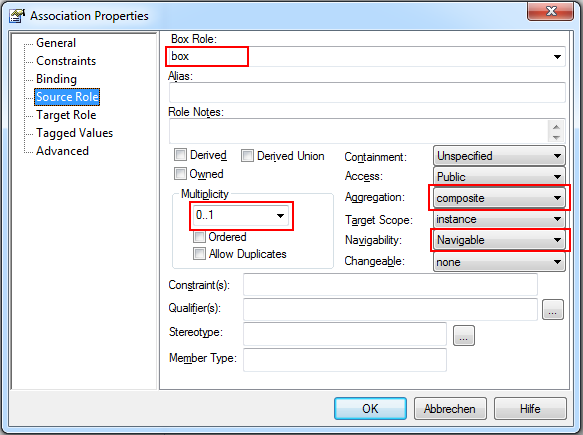
\includegraphics[width=0.9\textwidth]{ea_assocPropsSource}
	\caption{Properties for the source role of an EReference}
	\label{fig:role_source}
\end{figure}

\begin{figure}[htbp]
	\centering
	  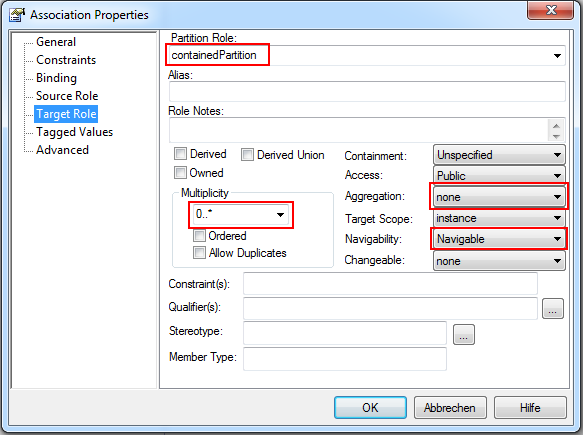
\includegraphics[width=0.9\textwidth]{ea_assocPropsTarget}
	\caption{Properties for the target role of an EReference}
	\label{fig:role_target}
\end{figure}

\end{itemize}

To review these properties, the first value you edited was the role name. The \texttt{Navigation} value should have been automatically set to
\texttt{Na\-vi\-ga\-ble}. Without these two settings, getter and setter methods will not be generated.

Next, you set the \texttt{Multiplicity} value.  In your source role (\texttt{Box}), you have allowed the creation of up to one target (\texttt{Partition})
reference for every connected source (\texttt{box}). This means you could not have a single target connected to two sources (i.e., one partition that belongs to
two boxes). In the target (\texttt{Partition}) role, you have specified that any source (in our case, \texttt{box}) can have any positive-sized number of targets.
Figure~\ref{fig:sketch_roles} sketches this schematically.

\vspace{0.5cm}

\begin{figure}[htbp]
	\centering
    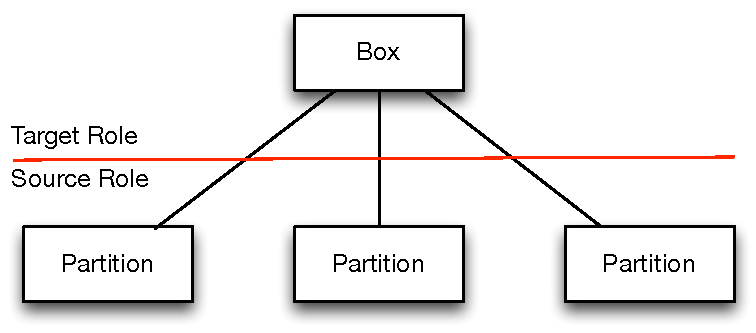
\includegraphics[width=0.6\textwidth]{sketch_multiplicities.pdf}
	\caption{The target and source roles of Leitner's Learning Box}
	\label{fig:sketch_roles}
\end{figure}
\FloatBarrier

Finally, you set the \texttt{Aggregation} value. In this case, \texttt{box} is a container for \texttt{Partition}s, and \texttt{containedPartition} is
consequently not.

\begin{itemize}
\item[$\blacktriangleright$] Take a moment to review how the \texttt{Aggregration} settings extend the \texttt{Multiplicity} rules. If you've done everything
right, your metamodel should now resemble Fig.~\ref{fig:ereference_completed}, with a single \emph{bidirectional EReference} between \texttt{Box} and
\texttt{Partition}.

\vspace{1cm}

\begin{figure}[htbp]
	\centering
  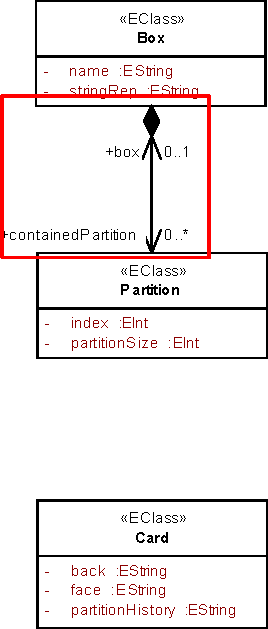
\includegraphics[width=0.35\textwidth]{ea_relationBoxPartition.pdf}
	\caption{\texttt{Box} contains \texttt{Partition}s}
	\label{fig:ereference_completed}
\end{figure}
\FloatBarrier

\item[$\blacktriangleright$] Following the same process, create two unidirectional self-EReferences for \texttt{Partition}, and then a second bidirectional
EReference\footnote{To be precise, \emph{all} EReferences in Ecore are actually unidirectional. A ``bidirectional'' EReference in our metamodel is really two
mapped EReferences that are opposites of each other. We however, believe it is simpler to handle these pairs as single EReferences, and prefer this
concise concrete syntax.} between \texttt{Partition} and \texttt{Card} (Fig.~\ref{fig:ereferences_all}). 

\vspace{1cm}

\begin{figure}[htbp]
	\centering
  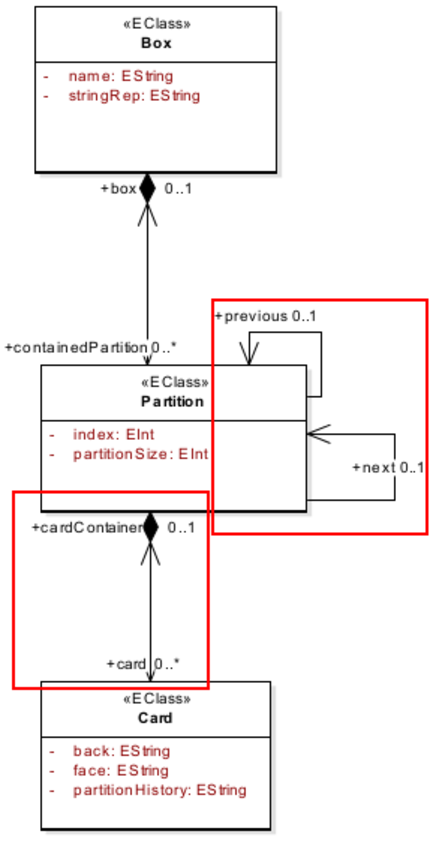
\includegraphics[width=0.7\textwidth]{ea_classAttributes}
	\caption{All relations in our metamodel}
	\label{fig:ereferences_all}
\end{figure}
\FloatBarrier

\vspace{1cm}

\item[$\blacktriangleright$] You'll notice that the connection between \texttt{Card} and \texttt{Partition} is similar to that between \texttt{Partition} and
\texttt{Box}. This makes sense as a partition should be able to hold an unlimited amount of cards, but a card can only belong to one partition at a time.

\vspace{1cm}

\item[$\blacktriangleright$] Export your diagram to Eclipse and refresh your workspace. Your Ecore file should now resemble Fig~\ref{fig:model_allClasses}.

\vspace{1cm}

\begin{figure}[htbp]
	\centering
  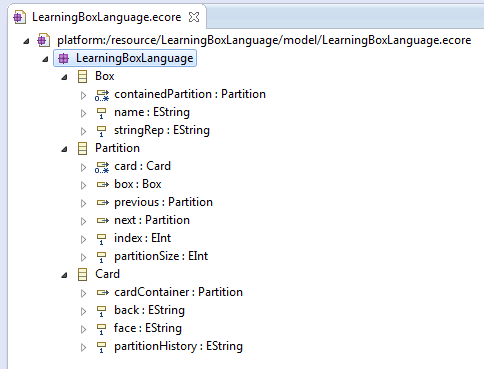
\includegraphics[width=0.7\textwidth]{eclipse_modelDeclaredClasses}
	\caption{Refreshed Ecore file with all EReferences}
	\label{fig:model_allClasses}
\end{figure}

\vspace{1cm}

\item[$\blacktriangleright$] All the required attributes and references for your learning box have now been set up. We encourage you to see how these are
declared in the textual syntax, starting on the immediate next page. In particular, check out Fig.~\ref{fig:allReferences}, where each EClass is fully
declared, and Fig.~\ref{fig:bothConstraints}, where bidirectionality is explicitly specified as a constraint.

\jumpSingle{static:methods vis}

\end{itemize}

\newpage
\subsubsection{Connecting your classes with MOSL}
\texHeader
\hypertarget{static:references tex}{}

In MOSL, the declaration of a reference is simple; the syntax is made up of four parts:  \small{\texttt{[Aggregation Type][Navigation
Name](Multiplicity):[Role]}}. A simple reference is defined with an arrow operator, while a contained reference is a sideways diamond and arrow combination.

% Edit me
To avoid redundancies in your code, it's important to know that both types automatically update the other role involved in the reference, which means you only
have to declare a direction once.


\begin{itemize}

\item[$\blacktriangleright$] Open \texttt{Box} class in the editor and add a \emph{container reference} named \texttt{containedPartition} with a multiplicity of zero
to infinite, of type \texttt{Partition} (Fig.~\ref{fig:cpartitionReference}). This means {\bf THAT}.

\begin{figure}[htbp]
	\centering
  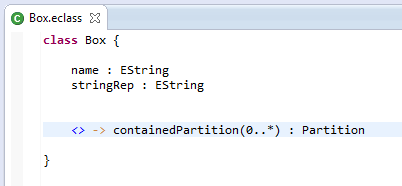
\includegraphics[width=0.6\textwidth]{eclass_box}
	\caption{Creating a \emph{contained reference} in \texttt{Box}}
	\label{fig:cpartitionReference}
\end{figure} 

\item[$\blacktriangleright$] Now add a \emph{simple reference} to \texttt{Partition}. Name it \texttt{box}, and allow it to hold up to one \texttt{Box}
(Fig.~\ref{fig:boxReference}). This means {\bf THAT}.

\begin{figure}[htbp]
	\centering
  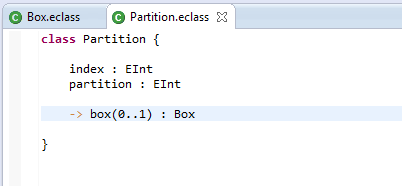
\includegraphics[width=0.6\textwidth]{eclass_partition}
	\caption{Creating a \emph{simple reference} in \texttt{Partition}}
	\label{fig:boxReference}
\end{figure} 

\item[$\blacktriangleright$] Congratulations, you have just built your first pair of EReferences. This pair is also known as a \emph{Bidirectional
EReference}! To see how this is depicted visually, check out Fig.~\ref{fig:ereference_completed} in the previous subsection.

\newpage

\item[$\blacktriangleright$] Now, lets create another EReference pair, or bidirectional EReference, between \texttt{Partition} and \texttt{Card}. If you think
about it, it's really not all that different than the relation between \texttt{Box} and \texttt{Partition}. In fact, it's not different at all! A
\texttt{Partition} should be able to hold an unlimited amount of \texttt{Card}s, but a \texttt{Card} should only be allowed to belong to zero or one
\texttt{Partition}s. Name the two new relations \texttt{containedPartition}, and \texttt{box}.

\item[$\blacktriangleright$] Your classes should now closely resemble Fig.~\ref{fig:almostAllReferences}.

\begin{figure}[htbp]
	\centering
  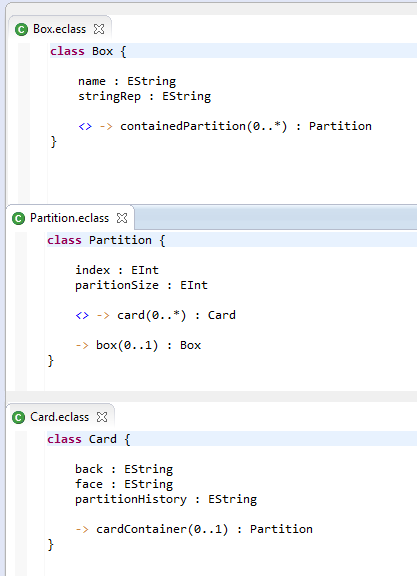
\includegraphics[width=0.65\textwidth]{eclipse_workspaceReferences}
	\caption{The Completed Bidirectional EReferences}
	\label{fig:almostAllReferences}
\end{figure} 

\item[$\blacktriangleright$] The next step is to set up two relations between \texttt{Partition} and itself, so it can shift between the previous and next
partition in the box. Create two new simple references, named \texttt{previous}, and \texttt{next}. Allow them to have a maximum of 1 link each.

\item[$\blacktriangleright$] All of our references are now set up! If you have done everything correctly, your classes should now resemble Fig.~\ref{fig:allReferences}.
To see how all of this is depicted visually, check out Fig.~\ref{fig:ereferences_all} in \hyperlink{sec:static vis}{section 2.1}.

\begin{figure}[htbp]
	\centering
  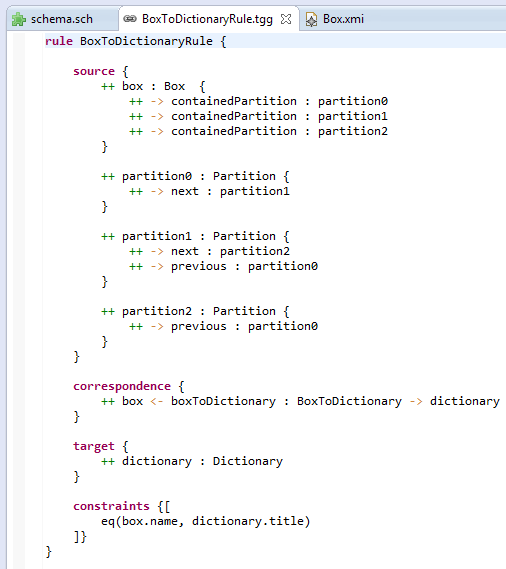
\includegraphics[width=0.6\textwidth]{eclipse_allReferences}
	\caption{All references in Leitner's Learning Box}
	\label{fig:allReferences}
\end{figure} 

\fancyfoot[R]{$\triangleright$ \hyperlink{static:methods tex}{Next}}
\end{itemize}



\newpage
\subsection{Method Signatures}
\genHeader
\hypertarget{static:methods vis}{}

To finish defining our types, lets define the \emph{signatures}\define{Operation Signature} of some operations that they'll eventually support.

\begin{stepbystep}

\item  Select \texttt{Partition} and either right-click to invoke the context-menu (\Cref{ea:add_operation})  and choose ``Features \&
Properties/Operations..'' or simply press \texttt{F10}.

\begin{figure}[htbp]
	\centering
  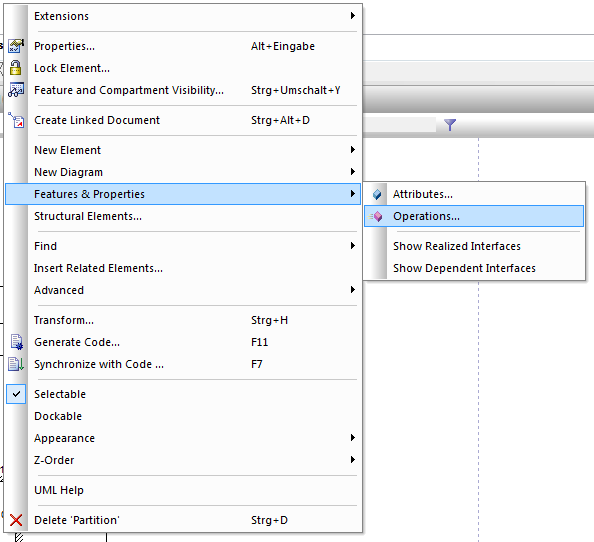
\includegraphics[width=0.8\textwidth]{../../org.moflon.doc.handbook.02_leitnersLearningBox/2_staticSemantics/4_creatingMethods/cmVisImages/ea_contextAddOperation}
	\caption{Add an operation}
	\label{ea:add_operation}
\end{figure}
\FloatBarrier

\item  In the dialogue that pops-up (\Cref{ea:operation_properties}), enter \texttt{empty} as the \texttt{Name} of the operation and \texttt{void} as the \texttt{Return Type}.

\vspace{0.5cm}

\item  In the same dialogue, click on \texttt{New Operation...} to add a second operation, \texttt{removeCard}, and edit the values as seen in 
\Cref{ea:operation_parameters}. Notice that the \texttt{Return Type} can be chosen by either the drop-down menu, or via direct typing. For types you've established in
the metamodel (e.g. \texttt{Card}) you have to use `\texttt{Select Type...}' from the drop-down menu.
\vspace{-.3cm}
\begin{quote}
{ \small
$\textbf{Very important:}$ Non-primitive types \emph{must} be chosen via `\texttt{Select Type...}' in the drop-down menu. It allows you to browse for the corresponding elements in
your project. Simply typing them won't work!
}
\end{quote}

\begin{figure}[htbp]
	\centering
  	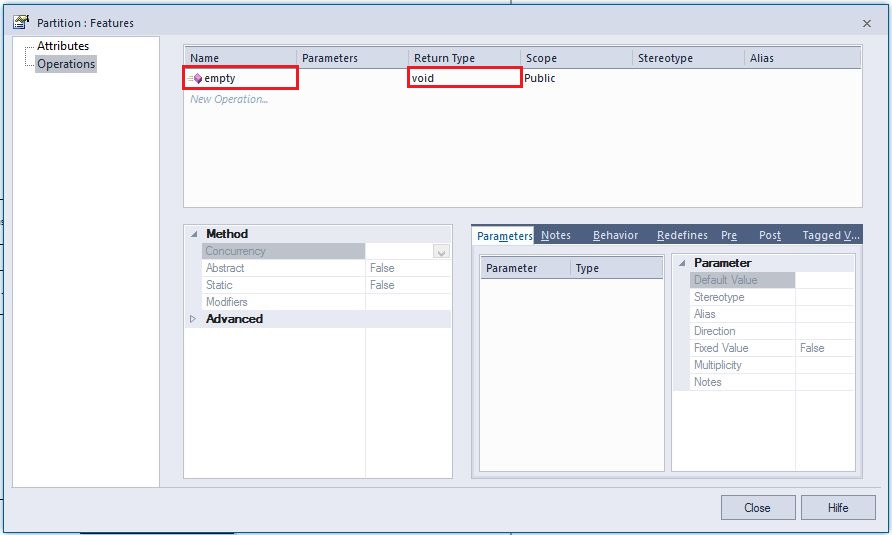
\includegraphics[width=\textwidth]{../../org.moflon.doc.handbook.02_leitnersLearningBox/2_staticSemantics/4_creatingMethods/cmVisImages/ea_operationEmpty}
	\caption{EClass properties editor}
	\label{ea:operation_properties}
\end{figure}


\item  Parameters can be added by selecting \texttt{Parameters} and
completing the dialouge (\Cref{ea:operation_parameters}). Please remember that you must also use either the drop-down menu, or direct typing to select the type or else validation
will fail.

\item  Repeat this process for the \texttt{check} operation (with the two parameters \texttt{card:Card, guess:EString}) that returns an \texttt{EBoolean}. 

\item  If you've done everything right, your dialogue should now contain three methods - \texttt{check}, \texttt{empty}, and
\texttt{removeCard} - each with the corresponding parameters and return types in \Cref{ea:operation_partition}.


\item  Add all operations analogously for \texttt{Box} and \texttt{Card} until your metamodel closely resembles
\Cref{ea:metamodel_complete}.\footnote{Please note that names of parameters may not be displayed by default in EA}

\item  To finish, export the metamodel for code generation in Eclipse, and examine the model once again. Each signature should have
appeared in their respective EClass.

\newpage

\vspace*{1cm}

\begin{figure}[htbp]
	\centering
  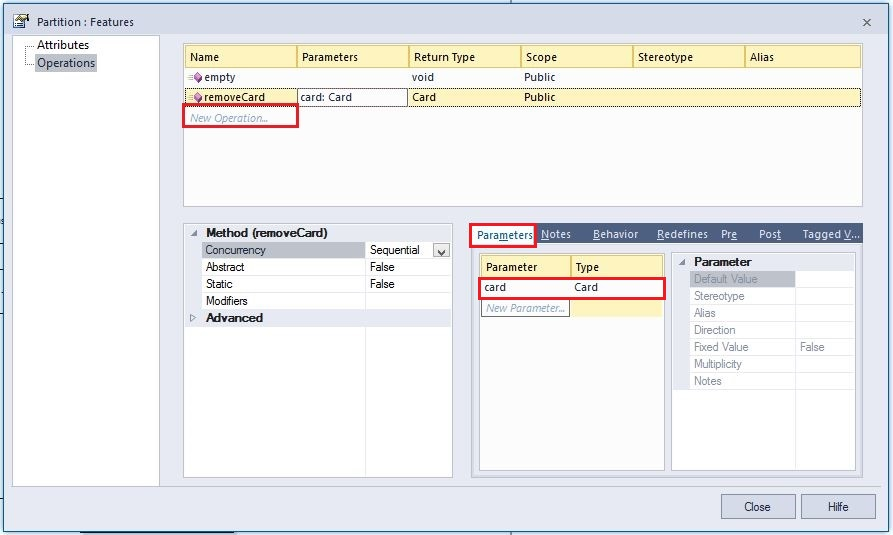
\includegraphics[width=\textwidth]{../../org.moflon.doc.handbook.02_leitnersLearningBox/2_staticSemantics/4_creatingMethods/cmVisImages/ea_operationRemoveCard}
	\caption{Parameters and return type}
	\label{ea:operation_parameters}
\end{figure}

\vspace{1cm}

\begin{figure}[h!]
	\centering
  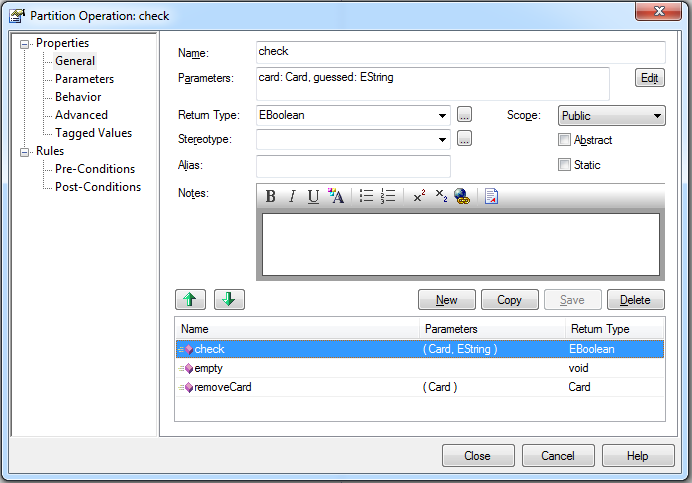
\includegraphics[width=\textwidth]{../../org.moflon.doc.handbook.02_leitnersLearningBox/2_staticSemantics/4_creatingMethods/cmVisImages/ea_operationCheck}
	\caption{All operations in \texttt{Partition}}
	\label{ea:operation_partition}
\end{figure}

\newpage


\begin{figure}[htbp]
	\centering
  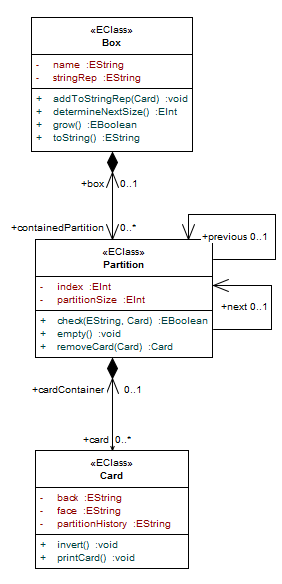
\includegraphics[width=0.6\textwidth]{../../org.moflon.doc.handbook.02_leitnersLearningBox/2_staticSemantics/4_creatingMethods/cmVisImages/ea_metamodelComplete}
\caption[Complete metamodel for our learning box.]{Complete metamodel for our learning box}
	\label{ea:metamodel_complete}
\end{figure}
\FloatBarrier

\end{stepbystep}


\newpage
\subsection{Method Signatures}
\texHeader
\hypertarget{static:methods tex}{}

\begin{itemize}

\item[$\blacktriangleright$] We're nearing the end of our model creation! One of the last things we need to do is to make the model \emph{do} something. After
all, a model that only stores attributes and references is a bit boring, right?

\item[$\blacktriangleright$] Let's set up the operations we want each EClass to do by declaring their \emph{signatures} which follow the syntax below:
\syntax{name `(' argument* `)' `:' return\_type \\
\\
With:\\
name, arguments, return\_type := STRING}

\item[$\blacktriangleright$] Starting with the \texttt{Partition} EClass, we want a partition to be able to do three things: compare the answer on a
\texttt{Card} with a guess and return a true/false response, remove a specific card from the partition, or empty itself of all cards.

\item[$\blacktriangleright$] Start with the \texttt{empty} method. It won't need any parameters, and it doesn't return anything. Declare this via:
\syntax{empty() : void}

\item[$\blacktriangleright$] Create two more functions for \texttt{Partition} the same way. We'll need a \texttt{removeCard} method that accepts and returns a
\texttt{Card}, as well as a EBoolean \texttt{check} method that accepts a \texttt{Card} and an \texttt{EString} guess. 

\item[$\blacktriangleright$] Your \texttt{Partition} EClass should now resemble Fig.~\ref{eclipse:partitionMethods}.

\vspace{0.5cm}

\begin{figure}[htbp]
	\centering
  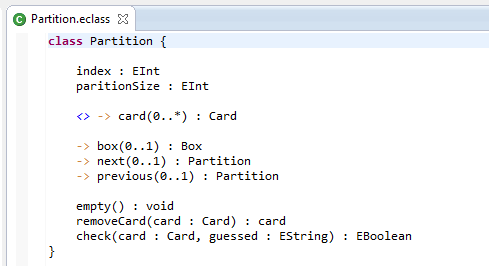
\includegraphics[width=0.6\textwidth]{eclipse_partitionMethods}
	\caption{The completed \texttt{Partition} EClass}
	\label{eclipse:partitionMethods}
\end{figure}

\vspace{0.5cm}

\item[$\blacktriangleright$] What needs to be done in the \texttt{Card} EClass? Well, in order to check the card, we'll need to be able to look at the flip
side. We'll also need to print whatever is on the current side. Create two paramater-less \texttt{void} functions, \texttt{invert} and \texttt{printCard}. 

\item[$\blacktriangleright$] Finally, what do we want to do with \texttt{Box}? In summary, we want a \texttt{Box} to:

\begin{description}
  \item[\texttt{determineNextSize():EInt}] Calculate how large a new partition in the box should be
  \item[\texttt{grow():EBoolean}] Increase the box by adding a new partition
  \item[\texttt{toString():EString}] Produce a string representation of the box with all its contents
  \item[\texttt{addToStringRep(card:Card):void}] Update the current string representation to include \texttt{card}
\end{description}

\item[$\blacktriangleright$] Implement the above signatures, and your entire workspace should now resemble Fig.~\ref{eclipse:workspaceMethods}.

\item[$\blacktriangleright$] Congratulations! You have now created a metamodel for our Learning Box using eMoflon's textual syntax! To see how
this looks in the visual syntax, check out Fig.~\ref{ea:metamodel_complete} from the previous section. As a final step, make sure you build the project and
wait for the package explorer to refresh. 

\newpage

\jumpSingle{validation tex}

\begin{figure}[htbp]
	\centering
  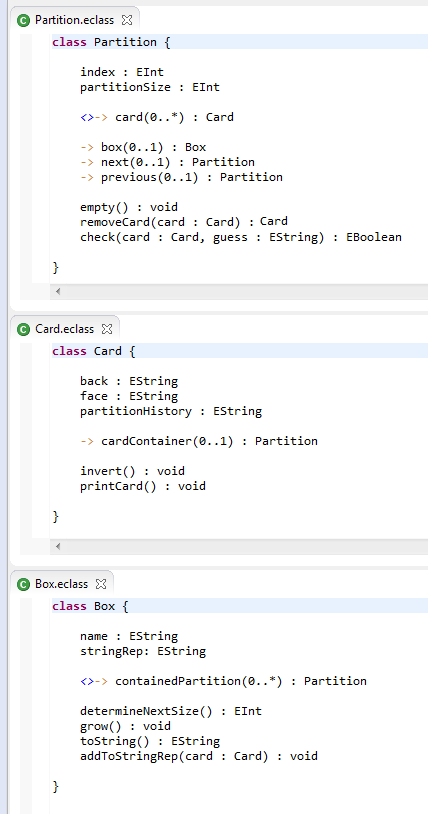
\includegraphics[width=0.7\textwidth]{eclipse_classesFullyDeclared}
	\caption{Completed method signatures}
	\label{eclipse:workspaceMethods}
\end{figure}
\FloatBarrier

\end{itemize}

\newpage
\genHeader
\hypertarget{validation vis}{} 
\subsection{eMoflon validation support in EA}
\label{sec:EAExport}

Our EA extension provides rudimentary support for validating your metamodel. Validation results are displayed and, in some cases, even ``quick fixes'' to
automatically solve the problems are offered. In addition to reviewing your model, the validation option automatically exports the current model to your eclipse
workspace if no problems were detected.

\begin{stepbystep}
\item If not already active, make the eMoflon control panel visible in EA by choosing ``Extensions/\-Add-In Windows''. This should
display a new output window, as depicted in \Cref{ea:validation_output}.
Many users prefer this interface as it provides quick access to all of eMoflon's features, as opposed to the drop down menu under ``Extensions/MOFLON::Ecore Addin" which only offers limited functionality.

\begin{figure}[htbp]
	\centering
  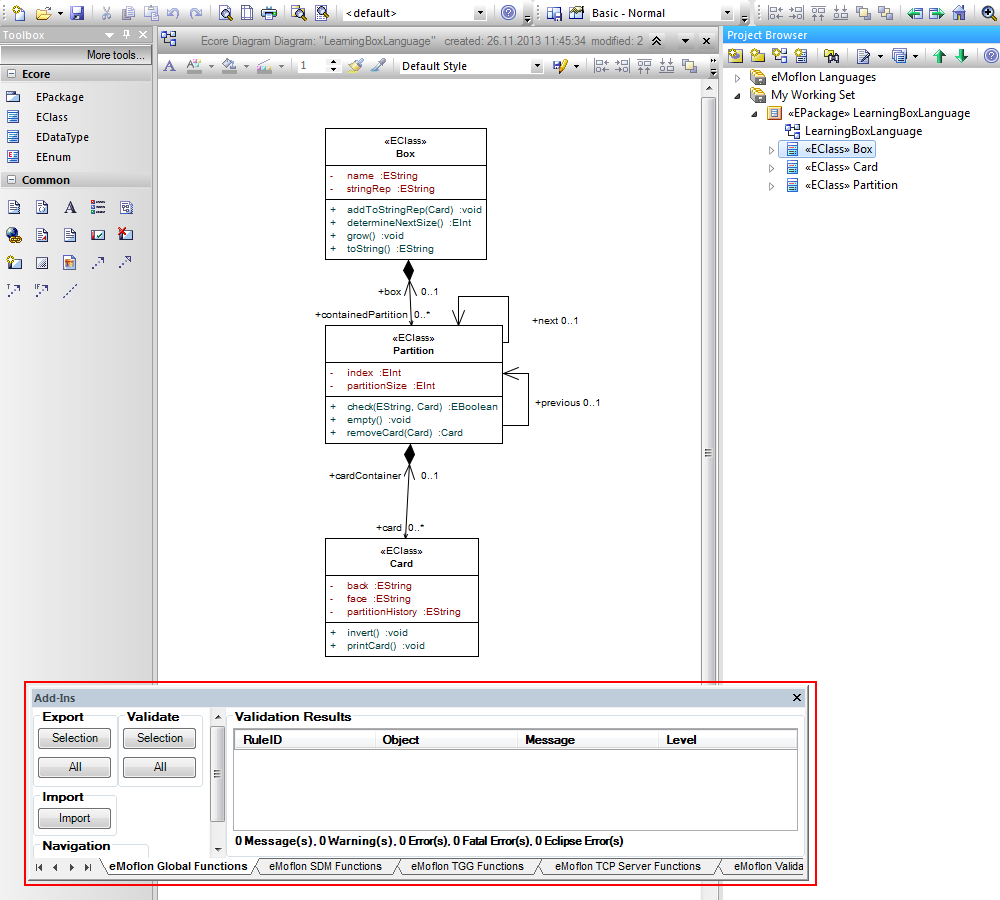
\includegraphics[width=\textwidth]{../../org.moflon.doc.handbook.02_leitnersLearningBox/2_staticSemantics/5_validation/images/ea_controlPanel}
	\caption{Activating the validation output window}
	\label{ea:validation_output}
\end{figure}
\FloatBarrier

\clearpage
\item To start the validation, choose ``Validate all'' in the ``Validate" section of the control panel
(\Cref{ea:validation_menu}). If you haven't made any mistakes while modelling your \texttt{LearningBoxLanguage} so far, the validation results window
should remain empty, indicating your metamodels are free of errors.

\begin{figure}[htbp]
	\centering
  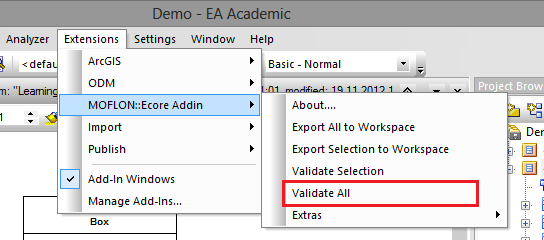
\includegraphics[width=1.0\textwidth]{../../org.moflon.doc.handbook.02_leitnersLearningBox/2_staticSemantics/5_validation/images/ea_startValidation}
	\caption{Starting the validation}
	\label{ea:validation_menu}
\end{figure}
\FloatBarrier
\end{stepbystep}

If an error did appear, the validation system attempts to suggest a ``Quick Fix.'' Why don't we examine the validation and quick fix features in detail? Let's
add two small modelling errors in \texttt{LearningBoxLanguage}.

\begin{stepbystep}
\item Create a new EClass in the \texttt{Learning\-Box\-Language} diagram. You can retain the default name \texttt{EClass1}. Let's
assume you wish to delete this class from your metamodel.

\item Select the rouge class in the diagram and press the \texttt{Delete} button on your keyboard. Note that this only deleted it from
the current diagram and \texttt{EClass1} still exists in the project browser (and thus in your metamodel).

\item Run the validation test, and notice the new \texttt{Information} message in the validation output.

This message informs you that \texttt{EClass1} is not on any diagram, and seeing as it is still in the metamodel, that this \emph{could} be a mistake. As you
can see, just pressing the \texttt{Delete} button is not the proper way of removing an EClass from a metamodel - It only removes it from the current
diagram!\footnote{Deleting elements properly and other EA specific aspects are discussed in detail in Part VI: Micellaneous}

\item Suppose you were inspecting a different diagram, and were not on the current screen. To navigate to the problematic element in the
\texttt{Project Browser}, click \emph{once} on the information message.

\item To check to see if there are any quick fixes available, \emph{double}-click the information message to invoke the ``QuickFix''
dialogue. In this case, there are two potential solutions - add the element to the current diagram or (properly) delete the element from the metamodel
(\Cref{ea:quick-fix1}). Since the latter was the original intent, click \texttt{Ok}.

\vspace{0.5cm}

\begin{figure}[htbp]
	\centering
  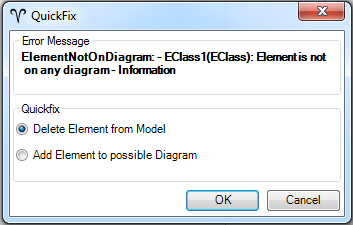
\includegraphics[width=0.55\textwidth]{../../org.moflon.doc.handbook.02_leitnersLearningBox/2_staticSemantics/5_validation/images/ea_quickFixElements}
	\caption{Quick fix for elements that are not on any diagram}
	\label{ea:quick-fix1}
\end{figure}
\FloatBarrier

\vspace{0.5cm}

\item \texttt{EClass1} should now be correctly removed from your metamodel. Your metamodel should now be error-free again as indicated by
the validation output window.

\item To make an error that leads to a more critical message than ``information,'' double-click the navigable EReference end
\texttt{previous} of the EClass \texttt{Partition}, and delete its role name as depicted in \Cref{ea:delete-role-name}. Affirm with \texttt{OK}.

\begin{figure}[htbp]
    \centering
  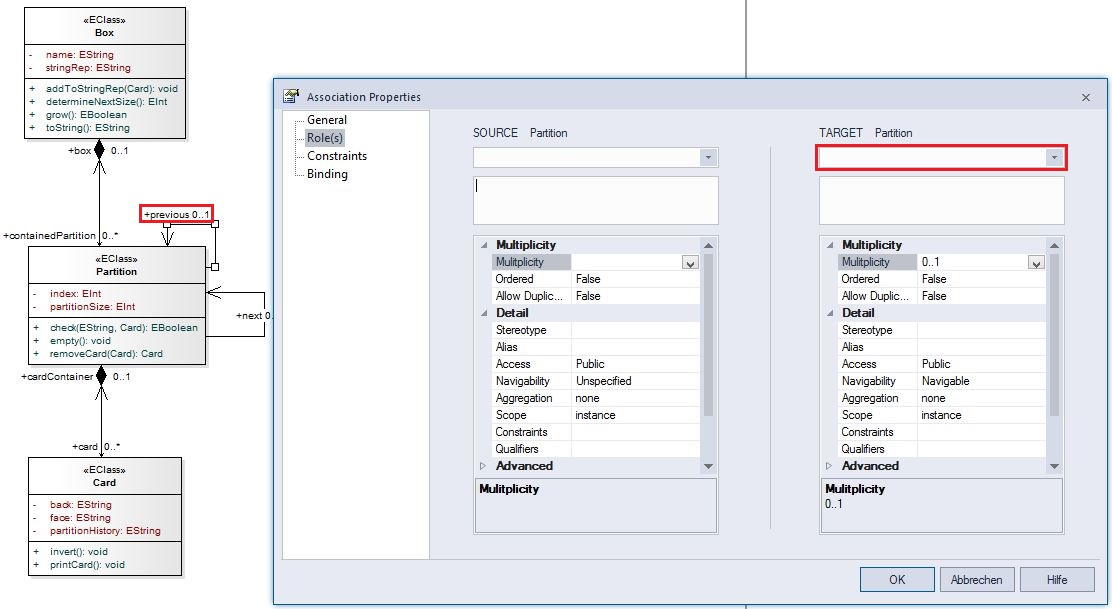
\includegraphics[width=1.0\textwidth]{../../org.moflon.doc.handbook.02_leitnersLearningBox/2_staticSemantics/5_validation/images/ea_validationDeleteRoleName}
    \caption{Deleting a navigable role name of an EReference}
    \label{ea:delete-role-name}
\end{figure}

\item You should now see a new \texttt{Fatal Error} in the validation output, stating that a navigable end \emph{must} have a role name.
Close all windows, then single click on the error once to open the relevant diagram and highlight the invalid element on the diagram. Double click the error to
view the quick fix menu (\Cref{ea:fatal-error}). As navigable references are mapped to data members in a Java class, omitting the name of a navigable
reference makes code generation impossible (data members ,i.e., class variables, must have a name).

\begin{figure}[htbp]
	\centering
  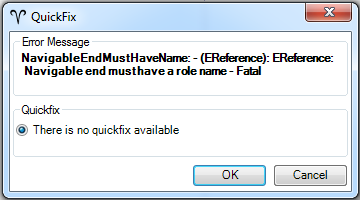
\includegraphics[width=0.6\textwidth]{../../org.moflon.doc.handbook.02_leitnersLearningBox/2_staticSemantics/5_validation/images/ea_quickFixFatal}
	\caption{Fatal error after deleting a navigable role name}
	\label{ea:fatal-error}
\end{figure}

\item Given there are no automatic solutions, correct your metamodel manually by setting the name of the navigable EReference back to
\texttt{previous}.

\item Ensure that your metamodel closely resembles \Cref{ea:metamodel_complete} again, and that there are no error messages before
proceeding.

\end{stepbystep}

\vspace*{1cm}

As you may have noticed, eMoflon distinguishes between five different types of validation messages:
\begin{description}
  \item[Information:]~\\
  This is only a hint for the user and can be safely ignored if you know what you're doing.
  Export and code generation should be possible, but certain naming/modelling conventions are violated, or a problematic situation has been detected.
  
  \item[Warning:]~\\ Export and code generation is possible, but only with defaults and automatic corrections applied by the code generator.
  As this might not be what the user wants, such cases are flagged as warnings (e.g., omitting the multiplicity at references which is automatically set by the
  code generator to 1).
  Being as explicit as possible is often better than relying on defaults.
  
  \item[Error:]~\\ Although the metamodel can be exported from EA, it is not Ecore conform, and code generation will not be possible.
 
  \item[Fatal Error:]~\\ The metamodel cannot be exported as required information, such as names or classifiers of model elements is incorrectly set or
  missing.
  
  \item[Eclipse Error:]~\\ Display error messages produced by our Eclipse plugin after an unsuccessful attempt to generate code. 

\end{description}

\newpage
\texHeader

{\bf \Large 3 \hspace{0.5cm}Validating Your Metamodel}

\subsection{ The MOSL Builder (Textual)}

\hypertarget{validation tex}{} Our MOSL language is accompanied with its own builder that proves support for validating the static semantics of your metamodel. Integrated with the Eclipse IDE, if there's an error in your files when you save, a message will appear in the console. Lets try to make an error, just to confirm it works.

Go to your \texttt{Partition} class and change the parameter type from \texttt{Card} to \texttt{card}. Press save. An error should immediately appear to inform you of your terrible mistake. Change your file back to the way it was, and the message should disappear.

Now, what would happen if you were to delete a reference? Can we make a more serious error appear? Go to any class, delete any reference, and press save. Nothing happens! As we mentioned earlier in the handbook, MOSL updates both classes and objects involved in any association. You won't ever have a 'hanging' link, or an issue where a link is defined in one place, but not another. 

\fancyfoot[R]{ $\triangleright$ \hyperlink{creatingInstance common}{Next step} }

\newpage 
\genHeader
\subsection{Reviewing your metamodel}
\hypertarget{static review}{}

Congratulations on completing the abstract syntax of your metamodel! Before moving on, lets take a step back and review. We have modelled a \texttt{Box} that
can contain an arbitrary amount of \texttt{Partition}s. A \texttt{Partition} in the \texttt{Box} has a \texttt{next} and \texttt{previous} \texttt{Partition}
that can or not be set. Finally, \texttt{Partition}s contain \texttt{Card}s.

A \texttt{Box} has a \texttt{name}, and can be extended by calling \texttt{grow}. A \texttt{Box} can print out its contents via the \texttt{toString} method.

The main method of the learning box is \texttt{Partition::check}, which takes a \texttt{Card} and the user's \texttt{EString} guess, and returns a \texttt{true}
or \texttt{false} value.

A \texttt{Partition} can also \texttt{remove} a specific \texttt{Card}, or empty itself of all  existing \texttt{Cards}. Last but not least, a
\texttt{Partition} has a \texttt{partitionSize} to indicate how many cards it currently has. Too many cards in the first partition could indicate that not
enough time has been dedicated to learning the terms. Too many near the end could show that the vocabulary set is too easy, and probably mastered.

A \texttt{Card} contains the actual content to be learned as a question on the card's \texttt{face} and the answer on the card's \texttt{back}. A \texttt{Card}s
also maintain \texttt{partition\-History}, which can be used to keep track of how often a \texttt{Card} has been answered incorrectly.
This may indicate how difficult the \texttt{Card} is for a specific user, and remind them to spend more time on that set. When learning a language, it makes
sense to be able to swap the target and source language and this is supported by \texttt{Card} via \texttt{invert} (turns the card around).

On a final note, we encourage you to review how the program was constructed in the syntax \emph{opposite} to the one you just used. Compare the differences
between modelling classes and references in diagrams using a separate program, then exporting to Eclipse to build, versus modelling entirely within the Eclipse
IDE with various commands. Which do you find easier to work with?

If you have had problems with this section, and, despite firmly believing everything is correct, things still don't work, feel free to contact us at 
\href{mailto:contact@moflon.org}{contact@moflon.org}.

\fancyfoot[R]{ $\triangleright$ \hyperlink{validation vis}{Next [visual]\hspace{0.2cm}} \\ $\triangleright$ \hyperlink{validation tex}{Next [textual]}}
 
